\documentclass{article}
\usepackage{float,amsmath}
\usepackage{graphicx}
\usepackage{color}
\usepackage[letterpaper,margin=1in]{geometry}
\usepackage{hyperref}

\usepackage{outlines}
\usepackage{enumitem}
\setenumerate[1]{label=\arabic*.}
\setenumerate[2]{label=\alph*.}
\setenumerate[3]{label=\arabic*.}
\setenumerate[4]{label=\roman*.}

\begin{document}

\author{HERA Software Team}
\title{Correlator Specification Tradeoffs}
\maketitle




\begin{figure}
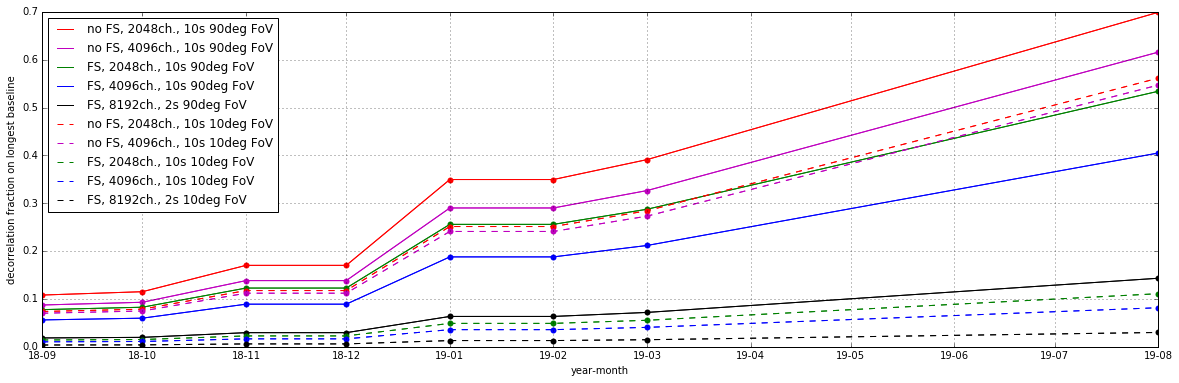
\includegraphics[width=\textwidth]{spec_calcs/decorrelation.png} 
\caption{Decorrelations on the longest baseline over the course of the buildout for various correlator options. The red line shows the current correlator specifications (2048 channels, 10s integration, no fringe stopping), the blue line shows the imaging-driven specifications (4096 channels, 10s integations with fringe stopping)for h2c and the magenta and green lines give two intermediate options. Finally, the black line shows the imaging-driven specification for the full array (8192 channels, 2s integrations with fringe stopping). Solid lines show the decorrelation at the horizon while the dashed lines show the decorrelation 10 degrees away from the zenith.}
\label{Fig:decorr}
\end{figure}

\begin{figure}
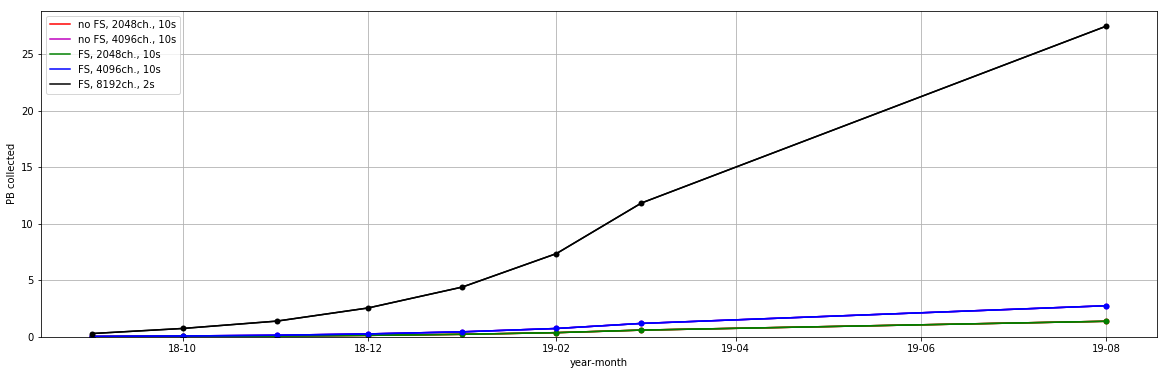
\includegraphics[width=\textwidth]{spec_calcs/corr_data_vols.png} 
\caption{Correlator data volumes on the longest baseline over the course of the buildout for various correlator options. The line colors are the same as in \ref{Fig:decorr}, but the red and green lines are on top of each other, as are the blue and magenta lines because the data rate depends only on the number of frequency channels and the final integration time (not on fringe stopping). The data volumes after RTP can be decreased substantially by baseline-dependent averaging.}
\label{Fig:corr_vol}
\end{figure}



\end{document}